\documentclass{chi-ext}
% Please be sure that you have the dependencies (i.e., additional LaTeX packages) to compile this example.
% See http://personales.upv.es/luileito/chiext/

%% EXAMPLE BEGIN -- HOW TO OVERRIDE THE DEFAULT COPYRIGHT STRIP -- (July 22, 2013 - Paul Baumann)
% \copyrightinfo{Permission to make digital or hard copies of all or part of this work for personal or classroom use is granted without fee provided that copies are not made or distributed for profit or commercial advantage and that copies bear this notice and the full citation on the first page. Copyrights for components of this work owned by others than ACM must be honored. Abstracting with credit is permitted. To copy otherwise, or republish, to post on servers or to redistribute to lists, requires prior specific permission and/or a fee. Request permissions from permissions@acm.org. \\
% {\emph{CHI'14}}, April 26--May 1, 2014, Toronto, Canada. \\
% Copyright \copyright~2014 ACM ISBN/14/04...\$15.00. \\
% DOI string from ACM form confirmation}
%% EXAMPLE END -- HOW TO OVERRIDE THE DEFAULT COPYRIGHT STRIP -- (July 22, 2013 - Paul Baumann)

\title{Drunken Ed ...}

\numberofauthors{6}
% Notice how author names are alternately typesetted to appear ordered in 2-column format;
% i.e., the first 4 autors on the first column and the other 4 auhors on the second column.
% Actually, it's up to you to strictly adhere to this author notation.
\author{
  \alignauthor{
  	\textbf{Alexander Biskupski}\\
  	\affaddr{AuthorCo, Inc.}\\
  	\affaddr{123 Author Ave.}\\
  	\affaddr{Authortown, PA 54321 USA}\\
  	\email{author1@anotherco.com}
  }\alignauthor{
  	\textbf{Marcel Karsten}\\
  	\affaddr{AuthorCo, Inc.}\\
  	\affaddr{123 Author Ave.}\\
  	\affaddr{Authortown, PA 54321 USA}\\
  	\email{author5@anotherco.com}
  }
  \vfil
  \alignauthor{
  	\textbf{Andreas Fender}\\
  	\affaddr{AuthorCo, Inc.}\\
  	\affaddr{123 Author Ave.}\\
  	\affaddr{Authortown, PA 54321 USA}\\
  	\email{author2@anotherco.com}
  }\alignauthor{
  	\textbf{Jonas Willaredt}\\
  	\affaddr{AuthorCo, Inc.}\\
  	\affaddr{123 Author Ave.}\\
  	\affaddr{Authortown, PA 54321 USA}\\
  	\email{author6@anotherco.com}
  }
  \vfil
  \alignauthor{
  	\textbf{Tiare Feuchtner}\\
  	\affaddr{AuthorCo, Inc.}\\
  	\affaddr{123 Author Ave.}\\
  	\affaddr{Authortown, PA 54321 USA}\\
  	\email{author3@anotherco.com}
  }
}

% Paper metadata (use plain text, for PDF inclusion and later re-using, if desired)
\def\plaintitle{CHI LaTeX Extended Abstracts Template}
\def\plainauthor{Luis A. Leiva}
\def\plainkeywords{Guides, instructions, author's kit, conference publications}
\def\plaingeneralterms{Documentation, Standardization}

\hypersetup{
  % Your metadata go here
  pdftitle={\plaintitle},
  pdfauthor={\plainauthor},  
  pdfkeywords={\plainkeywords},
  pdfsubject={\plaingeneralterms},
  % Quick access to color overriding:
  %citecolor=black,
  %linkcolor=black,
  %menucolor=black,
  %urlcolor=black,
}

\usepackage{graphicx}   % for EPS use the graphics package instead
\usepackage{balance}    % useful for balancing the last columns
\usepackage{bibspacing} % save vertical space in references

\usepackage{graphicx}

\newcommand{\drunkened}{\textit{Drunken Ed}}
\newcommand{\ed}{Ed}
\newcommand{\eds}{Ed's}
\newcommand{\lbreak}{\\[0.7cm]}

\newcommand{\image}[2]{
\begin{center}
\includegraphics[scale = #1]{pictures/#2}
\end{center}
}
\newcounter{imgcounter}
\newcommand{\figimage}[4]{
\begin{figure}[h] 
\image{#1}{#2}
\caption{\textit{#3}\\#4}
\label{#2}
\end{figure}
}
\newcommand{\capimage}[3]{
\begin{center}
\includegraphics[scale = #1]{#2}\\
\begin{small}#3\end{small}
\end{center}
}

\begin{document}

\maketitle

\begin{abstract}
In this sample we describe the formatting requirements for various SIGCHI related submissions 
and offer recommendations on writing for the worldwide SIGCHI readership. 
%Do not change the page size or page settings.
Please review this document even if you have submitted to SIGCHI conferences before, 
some format details have changed relative to previous years.
\end{abstract}

\keywords{\plainkeywords}
\textcolor{red}{Mandatory section to be included in your final version.}

\category{H.5.m}{Information interfaces and presentation (e.g., HCI)}{Miscellaneous}. 
%See \cite{ACMCCS} 
See: \url{http://www.acm.org/about/class/1998/} 
for help using the ACM Classification system.
\textcolor{red}{Mandatory section to be included in your final version.}

\terms{\plaingeneralterms}
\textcolor{red}{Optional section to be included in your final version.}


% =============================================================================
\section{Introduction}
% =============================================================================
\drunkened\ is a 2D balance game specifically designed for public displays. The player stands in front of a large display and is tracked by a Kinect. By bending his or her own upper body, the player steers a drunkyard called \textit{\ed}. The goal of the game is to walk as far as possible without falling down. While the time passes, the difficulty increases contineously. So the player has to keep the balance to not fall down, but at the same time, he or she has to hurry because it is getting harder and harder to increase the walked distance.\\
One key element of the visuals is the rotating camera: many balance games keep the world static while letting the player balance an object. In this game, the opposite is the case: it is the world around the figure, which needs to be balanced with respect to the upper body. 


%third person, but subjective

% =============================================================================
\section{Mechanics}
% =============================================================================
As long as no player stands in front of the screen, a bar is shown together with three blackboards containing the highscores. A hint invites the player to step onto the mark, which is located in front of the screen. When a player is detected, the main protagonist \ed appears. The player can now get used to the controls, without having to worry about balancing yet. At the same time, the player chooses the difficulty, encoded as three different alcoholic drinks: beer, wine and wodka. By bending him or herself, the player can move \ed\ to the respective drink. The user confirms his or her choice by doing a drink gesture.\lbreak

Afterwards, the main game starts. The player must make \ed\ walk as far as possible to the right. \ed\ does not walk in a controlled manner, but always follows his center of mass. This resembles a typical accentuated movement of a drunken person. The player bends his or her upper body to control \eds\ upper body, which in turn shifts his center of mass. \ed\ gets faster, the more he bends. The core mechanic is the rotating world: The upper body of \ed\ has the same orientation as of the player with respect to the screen, but not with respect to the rotating world around \ed. Therefore, the player must compensate the world's rotation to not tumble, which happens as soon as the angle between the upper body and the floor gets too narrow. Alternatively, \ed\ tumbles by getting to fast.\\
The higher the difficulty, the faster and uncontrollable the world rotates, which makes it hard to hold the balance and move to the right at the same time.\lbreak

\ed\ will eventually fall down. The game over overlay appears and the distance \ed\ walked until falling down is presented to the player. The distance is the score. If the player got a top three score, he or she can take a picture of him or herself to appear in the highscore list of the bar. The player does so by doing the drink gesture, in order that the picture captures him or her in a drinking posture. If the player does not want to take a picture, he or she has to wait for some seconds without doing anything or to leave the play area. Afterwards, the game restarts and the player gets back to the difficulty selection.\lbreak

During gameplay, the arms of \ed\ play an important role: In the difficulty selection, the arms are controllable by the players arms. However, in the main game, resembling typical cartoony postures of drunkyards, the arms are saggy, pointing straight towards the floor. Firstly, this emphasizes the loss of physical control, because the players arm movements are ignored now. Furthermore, they contribute to the players orientation, because \eds\ arms being aligned with the upper body mean a neutral posture without movement. When they are not aligned, the angle helps estimating the movement. In addition, the arms have an important feedback role: if \ed\ is getting too fast, they start to flail. If \ed\ is about to overbend, they start to swing. Players quickly understood those actions as alarming indicators.

% =============================================================================
\section{Design}
% =============================================================================
Since \drunkened\ is a public display game, it has to have several properties:
\begin{itemize}\compresslist
\item It must be very easy to understand and to play. Therefore, the game is reduced to one main input (the upper body) and one simple goal (walking to the right).
\item One game session must be quite short. The game and also public display games in general are targeting people, which are actually not planning to play. Therefore, they might not want to spent to much time with a game, that they started spontaneously. Furthermore, \drunkened\ is a single player game, so players have to take turns, which is easier with short game sessions.
\marginpar{
\begin{figure}
  \centering
  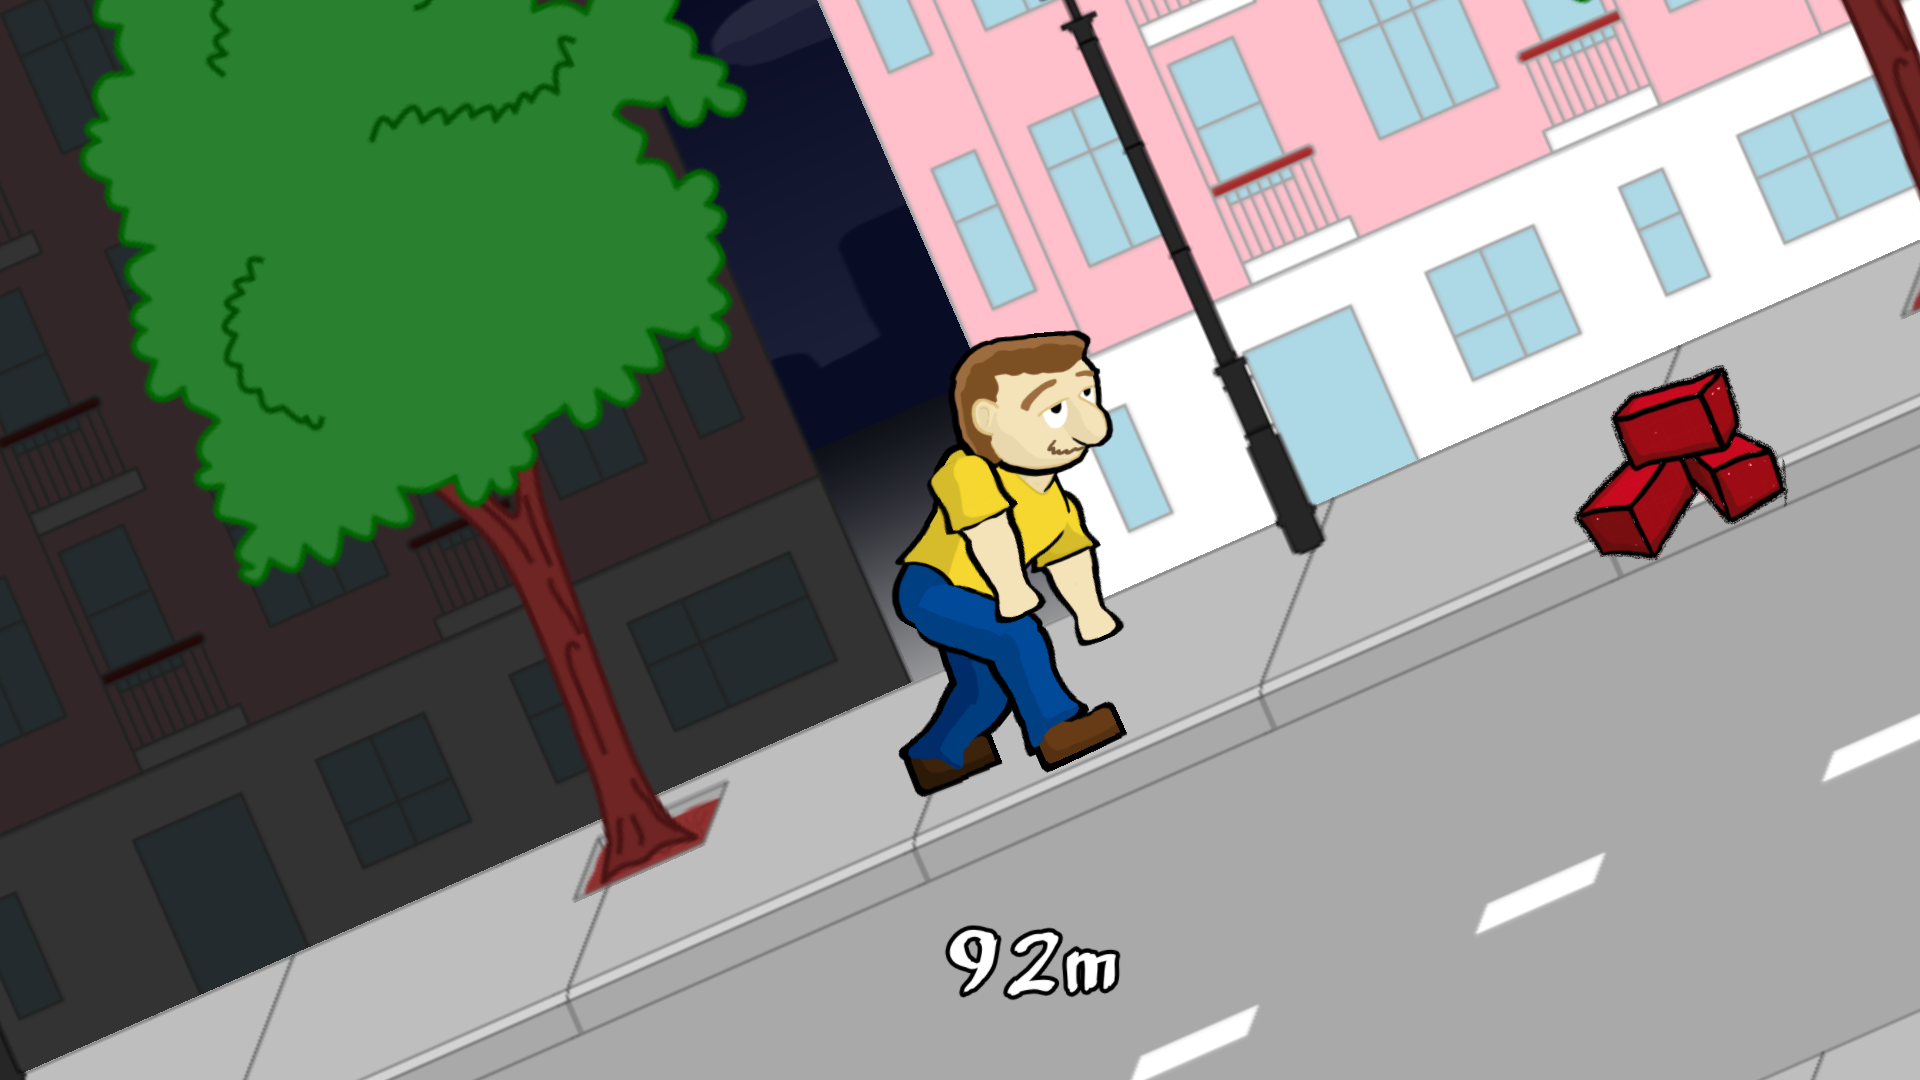
\includegraphics[width=\linewidth]{pictures/screenshot1.png}
  \caption{Insert a caption below each figure.}
  \label{fig:screenshot1}
\end{figure}
\begin{figure}
  \centering
  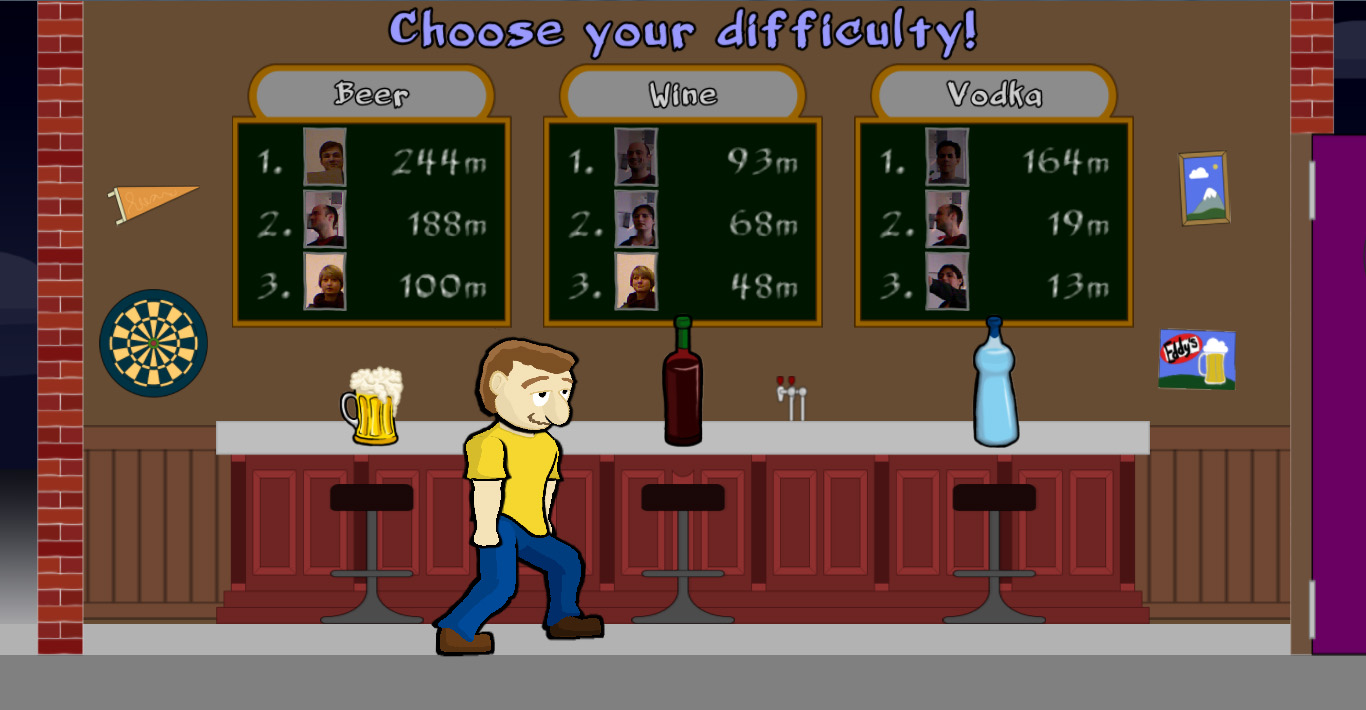
\includegraphics[width=\linewidth]{pictures/screenshot2.jpg}
  \caption{Insert a caption below each figure.}
  \label{fig:screenshot2}
\end{figure}
\begin{figure}
  \centering
  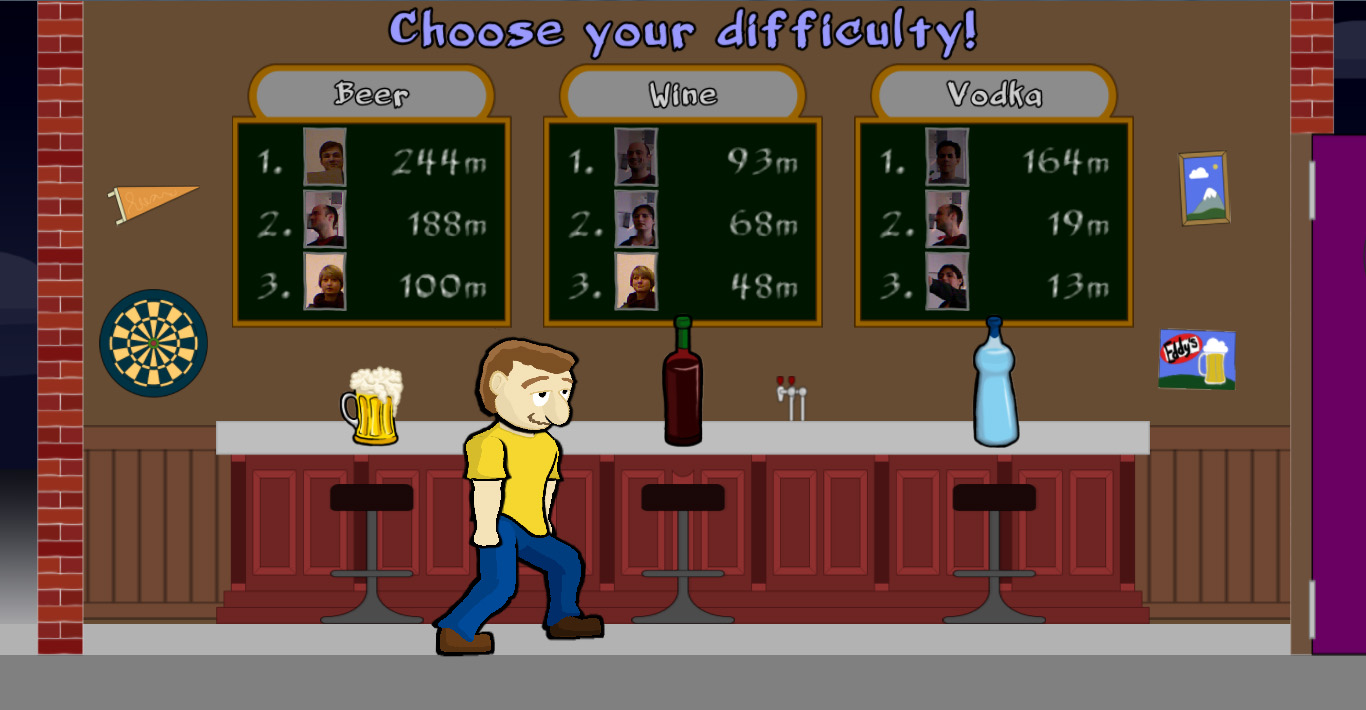
\includegraphics[width=\linewidth]{pictures/screenshot2.jpg}
  \caption{Insert a caption below each figure.}
  \label{fig:screenshot3}
\end{figure}
\begin{figure}
  \centering
  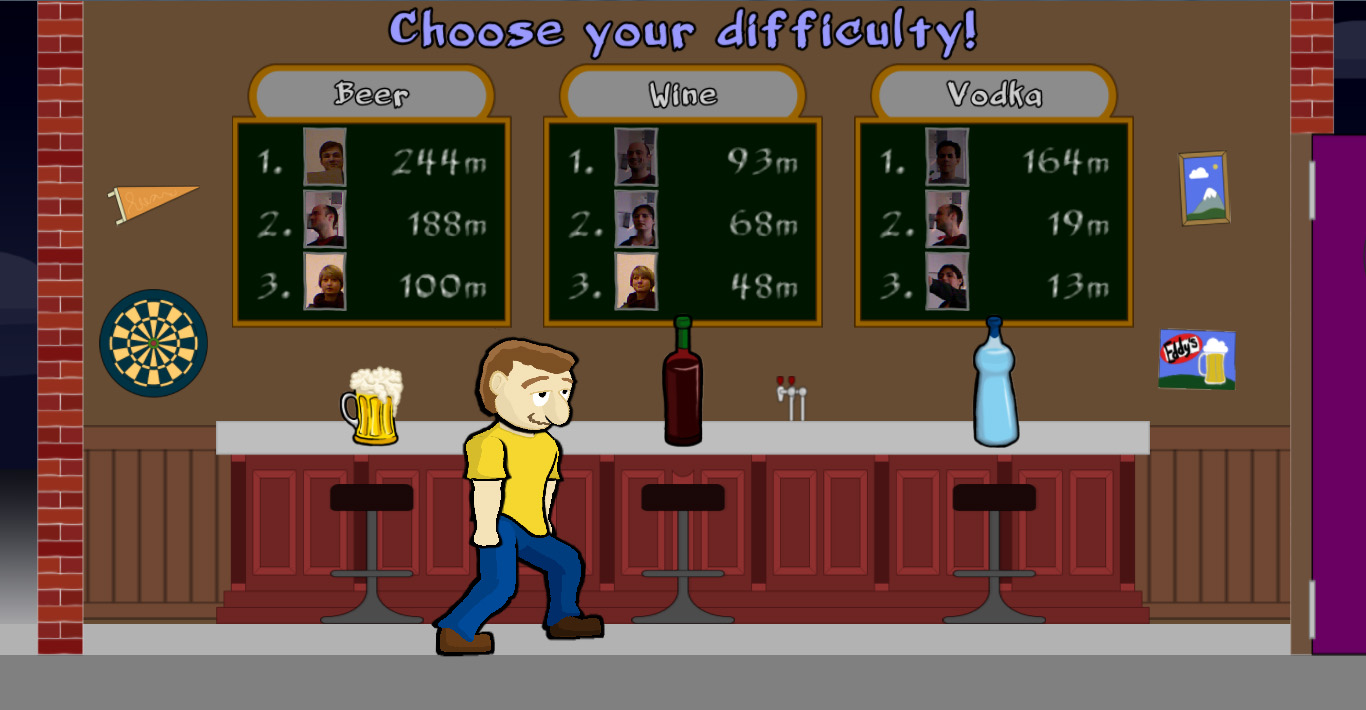
\includegraphics[width=\linewidth]{pictures/screenshot2.jpg}
  \caption{Insert a caption below each figure.}
  \label{fig:screenshot4}
\end{figure}
}
\item The narrative elements must be reduced to a minimum. There are no cutscenes, long texts etc. to tell the game's background. The animations, the players actions and keywords like ''distance'' give the game a humorous context.
\end{itemize}

\drunkened\ targets a joy of failing, that is, letting \ed\ eventually tumble and fall asleep. \eds\ tumbling is not implemented as an animation, but physics based, i.e. depending on \eds\ locomotion and angular velocity. This means, that failing varies from player to player, since they can take \ed\ into individual, often awkward, sleeping postures. This also attempts to compensate the fact, that \drunkened\ is a single player game, because spectators can have fun seeing others fail.

% =============================================================================
\section{Future work}
% =============================================================================
The game is still under development. Right now, placeholder graphics are replaced and new obstacle elements are added to enhance the gameplay.


% =============================================================================
\section{Template}
% =============================================================================

\begin{itemize}\compresslist
\item 	
Write in a straightforward style. 
Use simple sentence structure. 
Try to avoid long sentences and complex sentence structures. 
Use semicolons carefully.
\item 	
Use common and basic vocabulary (e.g., use the word ``unusual" rather than the word ``arcane").
\item 	
Briefly define or explain all technical terms. 
The terminology common to your practice/discipline may be different in other design practices/disciplines.
\item 	
Spell out all acronyms the first time they are used in your text. 
For example, ``World Wide Web (WWW)".
\item 	
Explain local references (e.g., not everyone knows all city names in a particular country).
\item 	
Explain ``insider" comments. 
Ensure that your whole audience understands any reference whose meaning you do not describe (e.g., do not assume that everyone has used a Macintosh or a particular application).
\item 	
Explain colloquial language and puns. 
Understanding phrases like ``red herring" requires a cultural knowledge of English. 
Humor and irony are difficult to translate.
\item 	
Use unambiguous forms for culturally localized concepts, such as times, dates, currencies and numbers (e.g., ``1-5-97" or ``5/1/97" may mean 5 January or 1 May, and ``seven o'clock" may mean 7:00 am or 19:00).
\item 	
Be careful with the use of gender-specific pronouns (he, she) and other gender-specific words (chairman, manpower, man-months). 
Use inclusive language (e.g., she or he, they, chair, staff, staff-hours, person-years) that is gender-neutral. 
If necessary, you may be able to use ``he" and ``she" in alternating sentences, so that the two genders occur equally often~\cite{Schwartz95}. 
\end{itemize}


% =============================================================================
\section{Figures}
% =============================================================================
The examples on this and following pages should help you get a feel for how screen-shots and other figures should be placed in the template. 
Be sure to make images large enough so the important details are legible and clear.

\begin{figure}
  \centering
  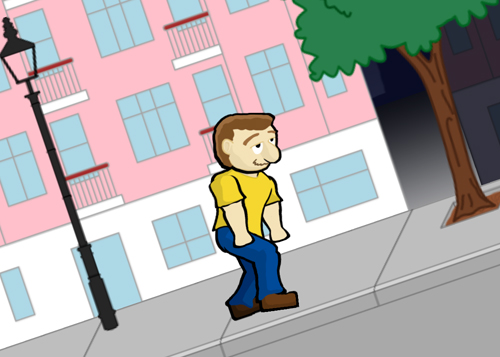
\includegraphics[width=\linewidth]{DrunkenEd.jpg}
  \caption{Insert a caption below each figure.}
  \label{fig:DrunkenEd}
\end{figure}

Your document may use color figures, which are included in the page limit; the figures must be usable when printed in black and white.
You can use the \LaTeX's \texttt{marginpar} command to insert figures in the (right) margin side of the document (see \autoref{fig:marginparsample}).


% =============================================================================
\section{References and Citations}
% =============================================================================
Use a numbered list of references at the end of the article, ordered alphabetically by first author, and referenced by numbers in brackets \cite{Anderson92,Klemmer02,Mather00,Zellweger01}
For papers from conference proceedings, include the title of the paper and an abbreviated name of the conference (e.g., for Interact 2003 proceedings, use Proc. Interact 2003). 
Do not include the location of the conference or the exact date; do include the page numbers if available. 
See the examples of citations at the end of this document. 

Your references should be published materials accessible to the public.  
Internal technical reports may be cited only if they are easily accessible (i.e., you provide the address for obtaining the report within your citation) and may be obtained by any reader for a nominal fee.  
Proprietary information may not be cited. 
Private communications should be acknowledged in the main text, not referenced  (e.g., [Robertson, personal communication]).

% =============================================================================
\section{Accessibility}
% =============================================================================
The Executive Council of SIGCHI has committed to making SIGCHI conferences more inclusive for researchers, practitioners, and educators with disabilities. As a part of this goal, the all authors are asked to work on improving the accessibility of their submissions. Specifically, we encourage authors to carry out the following five steps:
\begin{enumerate}
	\item Add alternative text to all figures
	\item Mark table headings
	\item Add tags to the PDF
	\item Verify the default language
	\item Set the tab order to ``Use Document Structure''
\end{enumerate}
Unfortunately good tools do not yet exist to create tagged PDF files from Latex. LaTeX users will need to carry out all of the above steps in the PDF directly using Adobe Acrobat, after the PDF has been generated.
 
For more information and links to instructions and resources, please see:
{\url{http://chi2014.acm.org/authors/guide-to-an-accessible-submission}}.

% =============================================================================
\section{Producing and testing PDF files}
% =============================================================================
We recommend that you produce a PDF version of your submission well before the final deadline. 
Besides making sure that you are able to produce a PDF, you will need to check that (a) the length of the file remains within the submission category's page limit, (b) the PDF file size is 4 megabytes or less, and (c) the file can be read and printed using Adobe Acrobat Reader. 
Test your PDF file by viewing or printing it with the same software we will use when we receive it, Adobe Acrobat Reader Version 7. 
This is widely available at no cost from~\cite{Acrobat7}.  
Note that most reviewers will use a North American/European version of Acrobat reader, which cannot handle documents containing non-North American or non-European fonts (e.g. Asian fonts).  
Please therefore do not use Asian fonts, and verify this by testing with a North American/European Acrobat reader (obtainable as above). Something as minor as including a space or punctuation character in a two-byte font can render a file unreadable.


% =============================================================================
\section{Dummy text}
% =============================================================================
Lorem ipsum dolor sit amet, consectetur adipiscing elit. Duis ut eros semper lectus vehicula elementum. Vestibulum ante ipsum primis in faucibus orci luctus et ultrices posuere cubilia Curae; Aliquam quis mi sapien. Suspendisse potenti. Mauris ultrices euismod velit sed dictum. Nullam auctor, nulla tincidunt dapibus suscipit, velit leo convallis metus, vel commodo libero erat in dolor. In laoreet porttitor ligula, porta blandit lectus consequat quis. 

Nam ut eros dui. Mauris volutpat elit metus, euismod pellentesque purus. In hac habitasse platea dictumst. Nullam consectetur lacinia interdum. Sed nec blandit nisi. Proin in nulla purus, sit amet iaculis tortor. Ut dapibus pellentesque nulla in interdum. Nunc at velit felis. Curabitur euismod neque eu orci varius in pharetra sem interdum. Morbi in mauris ac risus iaculis dapibus id in magna. Class aptent taciti sociosqu ad litora torquent per conubia nostra, per inceptos himenaeos.

\marginpar{
\begin{figure}
  \begin{center}
  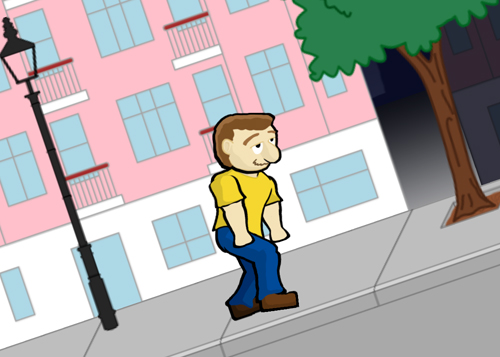
\includegraphics[width=\marginparwidth]{DrunkenEd.jpg}
  \caption{A marginal figure.}
  \label{fig:marginparsample}
  \end{center}  
\end{figure}
}
Aliquam consectetur quam sed odio varius vitae rhoncus urna fermentum. Phasellus viverra diam non justo porttitor varius. Integer ultrices accumsan lectus eget mollis. Nulla et leo sit amet nunc ornare rutrum sit amet ac dui. Cras vehicula accumsan purus nec fermentum. Mauris viverra condimentum metus, ut posuere quam laoreet nec. Phasellus massa tellus, ullamcorper nec porta sed, aliquet vitae nulla. Phasellus non tortor mauris. Cras ullamcorper egestas erat, vel rutrum elit viverra a. Donec in nisl ut est facilisis blandit. Quisque congue accumsan risus, ut venenatis magna vulputate vel. Nam commodo sapien vel mauris adipiscing nec dictum quam congue. Phasellus tempor vestibulum nisl quis blandit. Nullam condimentum auctor nibh, quis elementum libero tristique.



\section{Acknowledgements}
We thank all DUX 2003 publications support and staff who wrote this document originally and allowed us to modify it for this conference.
This template was based on Manas Tungare's \texttt{chi.cls}, and rewritten by Luis A. Leiva.

\section{References format}
References must be the same font size as other body text.
% REFERENCES FORMAT
% References must be the same font size as other body text.

\balance
\bibliographystyle{acm-sigchi}
\bibliography{DrunkenEd}

\end{document}